\subsection{Fits\-Image\-Array  Class Reference}
\label{class_fitsimagearray}\index{FitsImageArray@{Fits\-Image\-Array}}
Array of {\bf Image} {\rm (p.\,\pageref{class_image})} in a FITS file. 


{\tt \#include $<$fitsimagearray.h$>$}

Inheritance diagram for Fits\-Image\-Array::\begin{figure}[H]
\begin{center}
\leavevmode
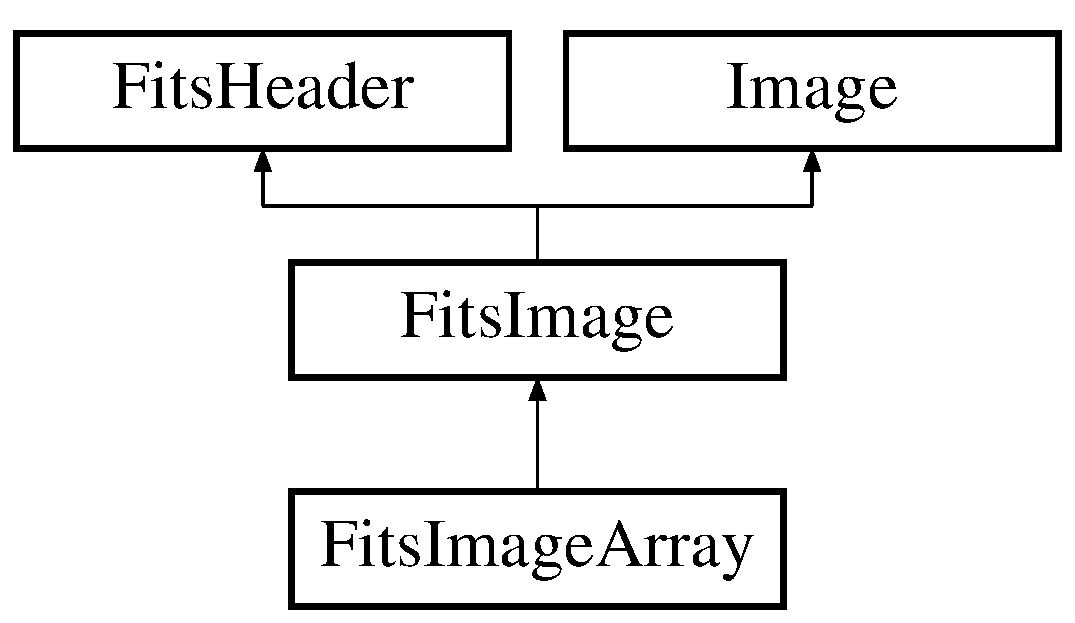
\includegraphics[height=3cm]{class_fitsimagearray}
\end{center}
\end{figure}
\subsubsection*{Public Types}
\begin{CompactItemize}
\item 
enum {\bf Status} \{ {\bf OK} =  0, 
{\bf OUTOFBOUNDS} =  1, 
{\bf FAILURE} =  2, 
{\bf ERRORWRITE} =  3, 
{\bf EMPTY} =  4
 \}
\begin{CompactList}\small\item\em Status flag for all functions.\item\end{CompactList}\item 
enum {\bf Criterion} \{ {\bf CHIP} =  1, 
{\bf FILTER} =  2, 
{\bf SIZE} =  4, 
{\bf EXTENDED} =  8
 \}
\begin{CompactList}\small\item\em Criterion fo image selection.\item\end{CompactList}\end{CompactItemize}
\subsubsection*{Public Methods}
\begin{CompactItemize}
\item 
{\bf Fits\-Image\-Array} (const string \&File\-Name, const Fits\-File\-Mode Mode=RO)
\begin{CompactList}\small\item\em Constructor for an existing fits image.\item\end{CompactList}\item 
{\bf Fits\-Image\-Array} (const string \&File\-Name, const {\bf Fits\-Header} \&header, bool Image\-In\-First\-HDU=true)
\begin{CompactList}\small\item\em Constructor for a new Fits\-Image\-Array with a minimal header from an existing {\bf Fits\-Header} {\rm (p.\,\pageref{class_fitsheader})}.\item\end{CompactList}\item 
{\bf Fits\-Image\-Array} (const string \&File\-Name, const {\bf Image} \&image, bool Image\-In\-First\-HDU=true)
\begin{CompactList}\small\item\em Constructor for a new Fits\-Image\-Array with a minimal header from an existing {\bf Image} {\rm (p.\,\pageref{class_image})}.\item\end{CompactList}\item 
\index{~FitsImageArray@{$\sim$FitsImageArray}!FitsImageArray@{Fits\-Image\-Array}}\index{FitsImageArray@{FitsImageArray}!~FitsImageArray@{$\sim$Fits\-Image\-Array}}
{\bf $\sim$Fits\-Image\-Array} ()\label{class_fitsimagearray_a3}

\begin{CompactList}\small\item\em Standard destructor.\item\end{CompactList}\item 
\index{Write@{Write}!FitsImageArray@{Fits\-Image\-Array}}\index{FitsImageArray@{FitsImageArray}!Write@{Write}}
{\bf Status} {\bf Write} (bool force\_\-bscale=false)\label{class_fitsimagearray_a4}

\begin{CompactList}\small\item\em Write all images to the FITS file.\item\end{CompactList}\item 
\index{SplitAndWrite@{SplitAndWrite}!FitsImageArray@{Fits\-Image\-Array}}\index{FitsImageArray@{FitsImageArray}!SplitAndWrite@{Split\-And\-Write}}
{\bf Status} {\bf Split\-And\-Write} (const string \&directory=\char`\"{}\char`\"{},int HDUMax=0)\label{class_fitsimagearray_a5}

\begin{CompactList}\small\item\em Write all images to separated FITS files (same as split\_\-fits).\item\end{CompactList}\item 
{\bf Status} {\bf Append} (const string \&filename)
\begin{CompactList}\small\item\em Add a {\bf Fits\-Image} {\rm (p.\,\pageref{class_fitsimage})} after the latest HDU.\item\end{CompactList}\item 
{\bf Status} {\bf Append} (const {\bf Image} \&image)
\begin{CompactList}\small\item\em Add an {\bf Image} {\rm (p.\,\pageref{class_image})} after the latest HDU.\item\end{CompactList}\item 
\index{At@{At}!FitsImageArray@{Fits\-Image\-Array}}\index{FitsImageArray@{FitsImageArray}!At@{At}}
{\bf Status} {\bf At} (int HDU)\label{class_fitsimagearray_a8}

\begin{CompactList}\small\item\em {\bf Point} {\rm (p.\,\pageref{class_point})} to the image at index HDU ( 1 $<$= HDU $<$= Get\-NImages()).\item\end{CompactList}\item 
\index{Next@{Next}!FitsImageArray@{Fits\-Image\-Array}}\index{FitsImageArray@{FitsImageArray}!Next@{Next}}
{\bf Status} {\bf Next} ()\label{class_fitsimagearray_a9}

\begin{CompactList}\small\item\em {\bf Point} {\rm (p.\,\pageref{class_point})} to the next image.\item\end{CompactList}\item 
void {\bf Set\-Criterion} (int value)
\begin{CompactList}\small\item\em Set the criterion for merging of {\bf Fits\-Image} {\rm (p.\,\pageref{class_fitsimage})}.\item\end{CompactList}\item 
\index{IsValid@{IsValid}!FitsImageArray@{Fits\-Image\-Array}}\index{FitsImageArray@{FitsImageArray}!IsValid@{Is\-Valid}}
bool {\bf Is\-Valid} ()\label{class_fitsimagearray_a11}

\begin{CompactList}\small\item\em Check whether this Fits\-Image\-Array is valid.\item\end{CompactList}\item 
\index{GetVersion@{GetVersion}!FitsImageArray@{Fits\-Image\-Array}}\index{FitsImageArray@{FitsImageArray}!GetVersion@{Get\-Version}}
string {\bf Get\-Version} ()\label{class_fitsimagearray_a12}

\begin{CompactList}\small\item\em Returns the version of this piece of code.\item\end{CompactList}\item 
bool {\bf Check\-Header} ({\bf Fits\-Header} \&header)
\begin{CompactList}\small\item\em Check whether header is consistent with f\-Main\-Header.\item\end{CompactList}\end{CompactItemize}


\subsubsection{Detailed Description}
Array of {\bf Image} {\rm (p.\,\pageref{class_image})} in a FITS file.

Inherites from {\bf Fits\-Image} {\rm (p.\,\pageref{class_fitsimage})} 



\subsubsection{Constructor \& Destructor Documentation}
\index{FitsImageArray@{Fits\-Image\-Array}!FitsImageArray@{FitsImageArray}}
\index{FitsImageArray@{FitsImageArray}!FitsImageArray@{Fits\-Image\-Array}}
\paragraph{\setlength{\rightskip}{0pt plus 5cm}Fits\-Image\-Array::Fits\-Image\-Array (const string \& {\em File\-Name}, const Fits\-File\-Mode {\em Mode} = RO)}\hfill\label{class_fitsimagearray_a0}


Constructor for an existing fits image.

\begin{CompactItemize}
\item 
 Opens in (Read\-Only (RO) mode by default, use RW to modify or create) \item 
 In RW mode, use this creator for an image already containing several images, i.e. with EXTEND=true (if EXTEND=false, {\bf Is\-Valid}() {\rm (p.\,\pageref{class_fitsimagearray_a11})}=false) \end{CompactItemize}
\index{FitsImageArray@{Fits\-Image\-Array}!FitsImageArray@{FitsImageArray}}
\index{FitsImageArray@{FitsImageArray}!FitsImageArray@{Fits\-Image\-Array}}
\paragraph{\setlength{\rightskip}{0pt plus 5cm}Fits\-Image\-Array::Fits\-Image\-Array (const string \& {\em File\-Name}, const {\bf Fits\-Header} \& {\em header}, bool {\em Image\-In\-First\-HDU} = true)}\hfill\label{class_fitsimagearray_a1}


Constructor for a new Fits\-Image\-Array with a minimal header from an existing {\bf Fits\-Header} {\rm (p.\,\pageref{class_fitsheader})}.

This header is used as a reference for image size, filter, chip. A criterion for accepting images can be set with the function Set\-Criterion  using the values of the enum {\bf Fits\-Image\-Array::Criterion} {\rm (p.\,\pageref{class_fitsimagearray_s10})}.  For instance Set\-Criterion(Fits\-Image\-Array::FILTER$|$Fits\-Image\-Array::CHIP) $<$=$>$ ask for the same filter and chip.\begin{Desc}
\item[{\bf Parameters: }]\par
\begin{description}
\item[
{\em Image\-In\-First\-HDU, if}]true (default) the first image that is added is saved in the first HDU, otherwise it is saved in the second one. \end{description}
\end{Desc}
\index{FitsImageArray@{Fits\-Image\-Array}!FitsImageArray@{FitsImageArray}}
\index{FitsImageArray@{FitsImageArray}!FitsImageArray@{Fits\-Image\-Array}}
\paragraph{\setlength{\rightskip}{0pt plus 5cm}Fits\-Image\-Array::Fits\-Image\-Array (const string \& {\em File\-Name}, const {\bf Image} \& {\em image}, bool {\em Image\-In\-First\-HDU} = true)}\hfill\label{class_fitsimagearray_a2}


Constructor for a new Fits\-Image\-Array with a minimal header from an existing {\bf Image} {\rm (p.\,\pageref{class_image})}.

This {\bf Image} {\rm (p.\,\pageref{class_image})} is used as a reference for image size (see previous constructor). The user can define other keys for accepting other images.\begin{Desc}
\item[{\bf Parameters: }]\par
\begin{description}
\item[
{\em Image\-In\-First\-HDU, if}]true (default) the first image that is added is saved in the first HDU, otherwise it is saved in the second one. \end{description}
\end{Desc}


\subsubsection{Member Function Documentation}
\index{FitsImageArray@{Fits\-Image\-Array}!Append@{Append}}
\index{Append@{Append}!FitsImageArray@{Fits\-Image\-Array}}
\paragraph{\setlength{\rightskip}{0pt plus 5cm}{\bf Status} Fits\-Image\-Array::Append (const {\bf Image} \& {\em image})}\hfill\label{class_fitsimagearray_a7}


Add an {\bf Image} {\rm (p.\,\pageref{class_image})} after the latest HDU.

\begin{Desc}
\item[{\bf Parameters: }]\par
\begin{description}
\item[
{\em Image}]that is appended. \begin{CompactItemize}
\item 
 A default {\bf Fits\-Header} {\rm (p.\,\pageref{class_fitsheader})} is written, namely with NAXIS$\ast$,  BSCALE, BZERO, BITPIX=16, and WRITEDAT \item 
 The user may add information to the header after the call to this function \end{CompactItemize}
\end{description}
\end{Desc}
\index{FitsImageArray@{Fits\-Image\-Array}!Append@{Append}}
\index{Append@{Append}!FitsImageArray@{Fits\-Image\-Array}}
\paragraph{\setlength{\rightskip}{0pt plus 5cm}{\bf Status} Fits\-Image\-Array::Append (const string \& {\em filename})}\hfill\label{class_fitsimagearray_a6}


Add a {\bf Fits\-Image} {\rm (p.\,\pageref{class_fitsimage})} after the latest HDU.

\begin{Desc}
\item[{\bf Parameters: }]\par
\begin{description}
\item[
{\em filename, name}]of the fits file to append Uses cfitsio fits\_\-copy\_\-hdu, i.e. toads is not used a lot except for checking the compatibility of {\bf Fits\-Header} {\rm (p.\,\pageref{class_fitsheader})} \end{description}
\end{Desc}
\index{FitsImageArray@{Fits\-Image\-Array}!CheckHeader@{CheckHeader}}
\index{CheckHeader@{CheckHeader}!FitsImageArray@{Fits\-Image\-Array}}
\paragraph{\setlength{\rightskip}{0pt plus 5cm}bool Fits\-Image\-Array::Check\-Header ({\bf Fits\-Header} \& {\em header})}\hfill\label{class_fitsimagearray_a13}


Check whether header is consistent with f\-Main\-Header.

\begin{CompactItemize}
\item 
 Used by {\bf Fits\-Image\-Array::Append} {\rm (p.\,\pageref{class_fitsimagearray_a6})} \item 
 Uses f\-Selected\-Criterion (see Set\-Criterion) \end{CompactItemize}
\index{FitsImageArray@{Fits\-Image\-Array}!SetCriterion@{SetCriterion}}
\index{SetCriterion@{SetCriterion}!FitsImageArray@{Fits\-Image\-Array}}
\paragraph{\setlength{\rightskip}{0pt plus 5cm}void Fits\-Image\-Array::Set\-Criterion (int {\em value})\hspace{0.3cm}{\tt  [inline]}}\hfill\label{class_fitsimagearray_a10}


Set the criterion for merging of {\bf Fits\-Image} {\rm (p.\,\pageref{class_fitsimage})}.

\begin{Desc}
\item[{\bf Parameters: }]\par
\begin{description}
\item[
{\em value}]: example Fits\-Image\-Array::CHIP$|$Fits\-Image\-Array::FILTER \end{description}
\end{Desc}


The documentation for this class was generated from the following file:\begin{CompactItemize}
\item 
{\bf fitsimagearray.h}\end{CompactItemize}
